\documentclass[1p]{elsarticle_modified}
%\bibliographystyle{elsarticle-num}

%\usepackage[colorlinks]{hyperref}
%\usepackage{abbrmath_seonhwa} %\Abb, \Ascr, \Acal ,\Abf, \Afrak
\usepackage{amsfonts}
\usepackage{amssymb}
\usepackage{amsmath}
\usepackage{amsthm}
\usepackage{scalefnt}
\usepackage{amsbsy}
\usepackage{kotex}
\usepackage{caption}
\usepackage{subfig}
\usepackage{color}
\usepackage{graphicx}
\usepackage{xcolor} %% white, black, red, green, blue, cyan, magenta, yellow
\usepackage{float}
\usepackage{setspace}
\usepackage{hyperref}

\usepackage{tikz}
\usetikzlibrary{arrows}

\usepackage{multirow}
\usepackage{array} % fixed length table
\usepackage{hhline}

%%%%%%%%%%%%%%%%%%%%%
\makeatletter
\renewcommand*\env@matrix[1][\arraystretch]{%
	\edef\arraystretch{#1}%
	\hskip -\arraycolsep
	\let\@ifnextchar\new@ifnextchar
	\array{*\c@MaxMatrixCols c}}
\makeatother %https://tex.stackexchange.com/questions/14071/how-can-i-increase-the-line-spacing-in-a-matrix
%%%%%%%%%%%%%%%

\usepackage[normalem]{ulem}

\newcommand{\msout}[1]{\ifmmode\text{\sout{\ensuremath{#1}}}\else\sout{#1}\fi}
%SOURCE: \msout is \stkout macro in https://tex.stackexchange.com/questions/20609/strikeout-in-math-mode

\newcommand{\cancel}[1]{
	\ifmmode
	{\color{red}\msout{#1}}
	\else
	{\color{red}\sout{#1}}
	\fi
}

\newcommand{\add}[1]{
	{\color{blue}\uwave{#1}}
}

\newcommand{\replace}[2]{
	\ifmmode
	{\color{red}\msout{#1}}{\color{blue}\uwave{#2}}
	\else
	{\color{red}\sout{#1}}{\color{blue}\uwave{#2}}
	\fi
}

\newcommand{\Sol}{\mathcal{S}} %segment
\newcommand{\D}{D} %diagram
\newcommand{\A}{\mathcal{A}} %arc


%%%%%%%%%%%%%%%%%%%%%%%%%%%%%5 test

\def\sl{\operatorname{\textup{SL}}(2,\Cbb)}
\def\psl{\operatorname{\textup{PSL}}(2,\Cbb)}
\def\quan{\mkern 1mu \triangleright \mkern 1mu}

\theoremstyle{definition}
\newtheorem{thm}{Theorem}[section]
\newtheorem{prop}[thm]{Proposition}
\newtheorem{lem}[thm]{Lemma}
\newtheorem{ques}[thm]{Question}
\newtheorem{cor}[thm]{Corollary}
\newtheorem{defn}[thm]{Definition}
\newtheorem{exam}[thm]{Example}
\newtheorem{rmk}[thm]{Remark}
\newtheorem{alg}[thm]{Algorithm}

\newcommand{\I}{\sqrt{-1}}
\begin{document}

%\begin{frontmatter}
%
%\title{Boundary parabolic representations of knots up to 8 crossings}
%
%%% Group authors per affiliation:
%\author{Yunhi Cho} 
%\address{Department of Mathematics, University of Seoul, Seoul, Korea}
%\ead{yhcho@uos.ac.kr}
%
%
%\author{Seonhwa Kim} %\fnref{s_kim}}
%\address{Center for Geometry and Physics, Institute for Basic Science, Pohang, 37673, Korea}
%\ead{ryeona17@ibs.re.kr}
%
%\author{Hyuk Kim}
%\address{Department of Mathematical Sciences, Seoul National University, Seoul 08826, Korea}
%\ead{hyukkim@snu.ac.kr}
%
%\author{Seokbeom Yoon}
%\address{Department of Mathematical Sciences, Seoul National University, Seoul, 08826,  Korea}
%\ead{sbyoon15@snu.ac.kr}
%
%\begin{abstract}
%We find all boundary parabolic representation of knots up to 8 crossings.
%
%\end{abstract}
%\begin{keyword}
%    \MSC[2010] 57M25 
%\end{keyword}
%
%\end{frontmatter}

%\linenumbers
%\tableofcontents
%
\newcommand\colored[1]{\textcolor{white}{\rule[-0.35ex]{0.8em}{1.4ex}}\kern-0.8em\color{red} #1}%
%\newcommand\colored[1]{\textcolor{white}{ #1}\kern-2.17ex	\textcolor{white}{ #1}\kern-1.81ex	\textcolor{white}{ #1}\kern-2.15ex\color{red}#1	}

{\Large $\underline{12n_{0611}~(K12n_{0611})}$}

\setlength{\tabcolsep}{10pt}
\renewcommand{\arraystretch}{1.6}
\vspace{1cm}\begin{tabular}{m{100pt}>{\centering\arraybackslash}m{274pt}}
\multirow{5}{120pt}{
	\centering
	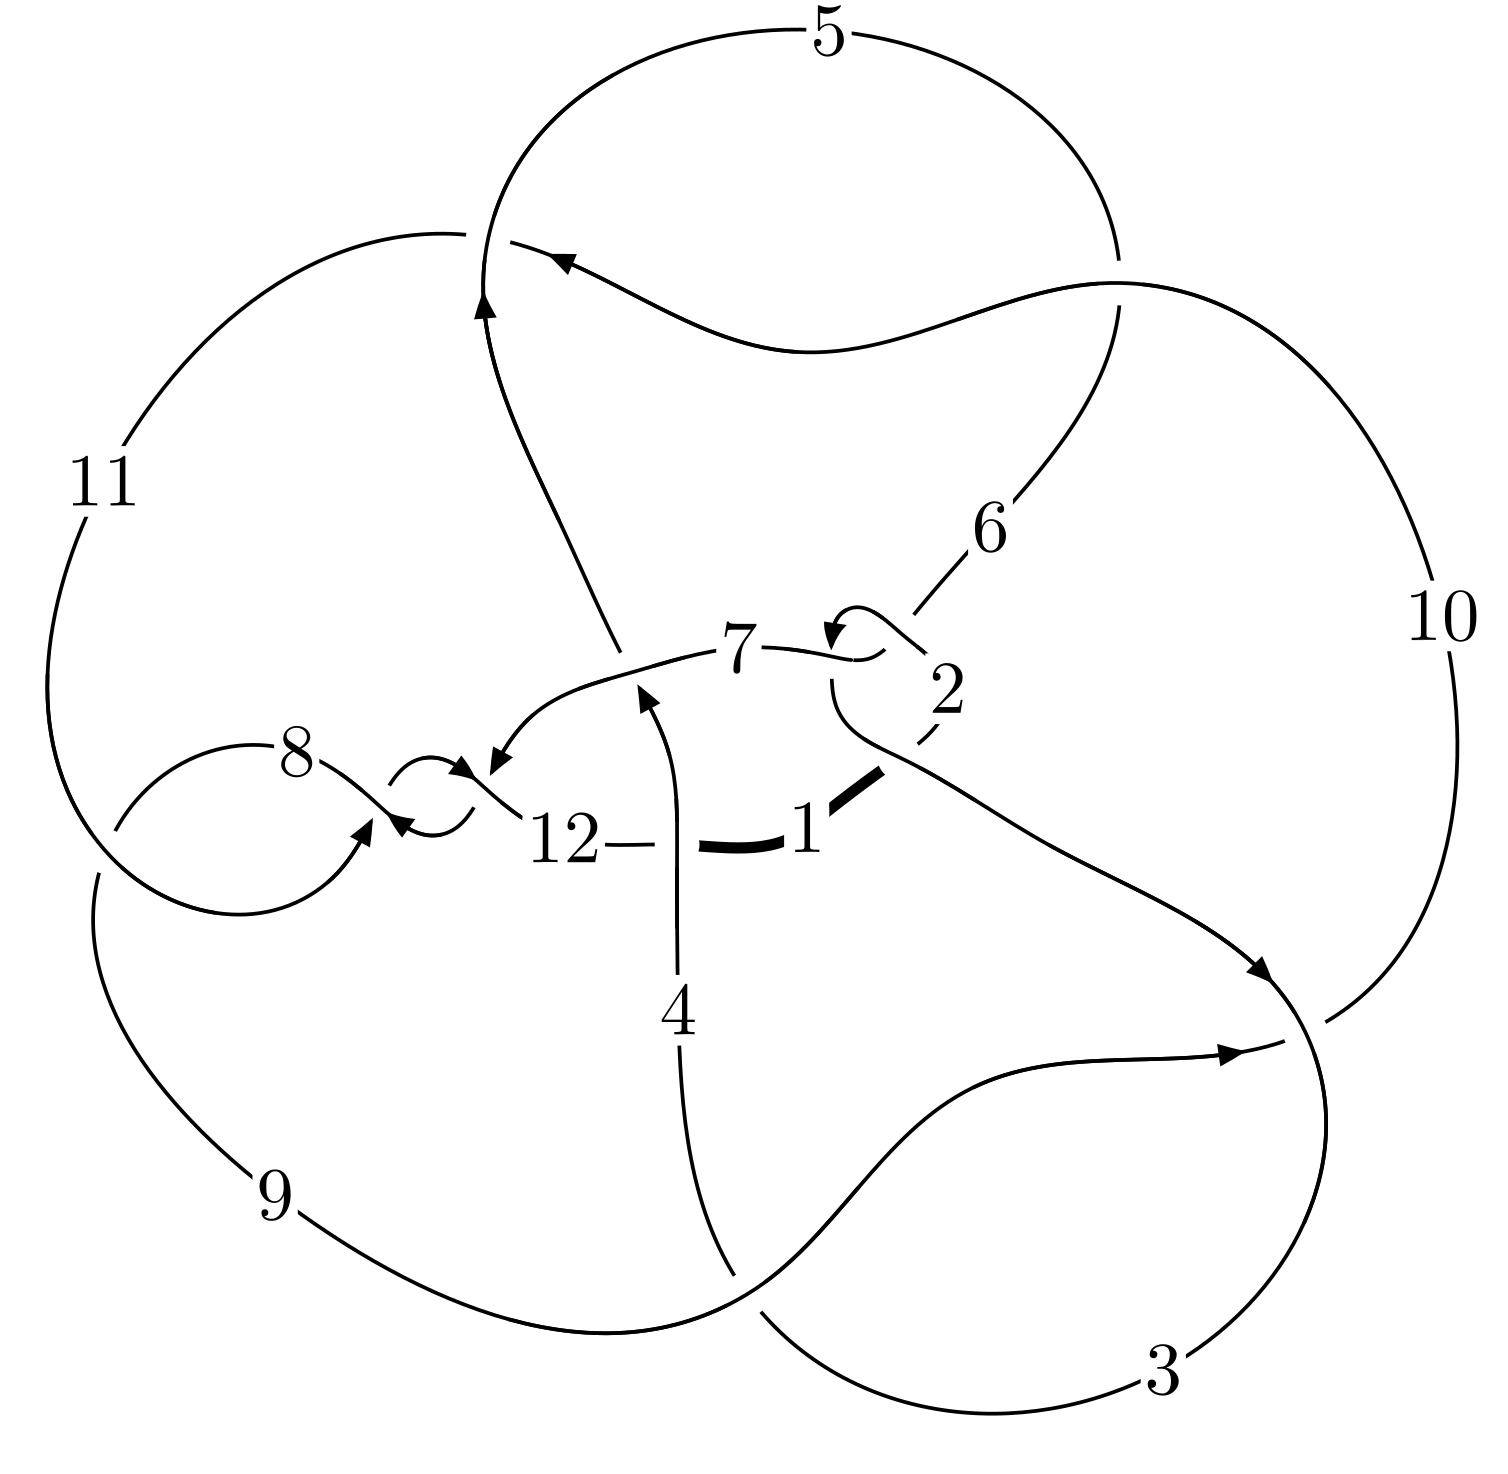
\includegraphics[width=112pt]{../../../GIT/diagram.site/Diagrams/png/2700_12n_0611.png}\\
\ \ \ A knot diagram\footnotemark}&
\allowdisplaybreaks
\textbf{Linearized knot diagam} \\
\cline{2-2}
 &
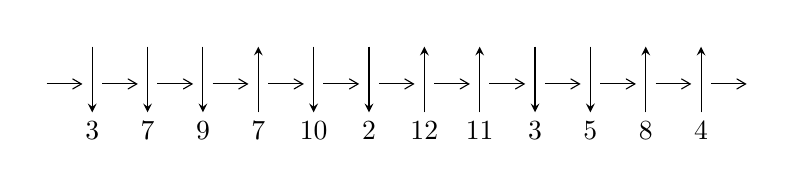
\begin{tikzpicture}[x=20pt, y=17pt]
	% nodes
	\node (C0) at (0, 0) {};
	\node (C1) at (1, 0) {};
	\node (C1U) at (1, +1) {};
	\node (C1D) at (1, -1) {3};

	\node (C2) at (2, 0) {};
	\node (C2U) at (2, +1) {};
	\node (C2D) at (2, -1) {7};

	\node (C3) at (3, 0) {};
	\node (C3U) at (3, +1) {};
	\node (C3D) at (3, -1) {9};

	\node (C4) at (4, 0) {};
	\node (C4U) at (4, +1) {};
	\node (C4D) at (4, -1) {7};

	\node (C5) at (5, 0) {};
	\node (C5U) at (5, +1) {};
	\node (C5D) at (5, -1) {10};

	\node (C6) at (6, 0) {};
	\node (C6U) at (6, +1) {};
	\node (C6D) at (6, -1) {2};

	\node (C7) at (7, 0) {};
	\node (C7U) at (7, +1) {};
	\node (C7D) at (7, -1) {12};

	\node (C8) at (8, 0) {};
	\node (C8U) at (8, +1) {};
	\node (C8D) at (8, -1) {11};

	\node (C9) at (9, 0) {};
	\node (C9U) at (9, +1) {};
	\node (C9D) at (9, -1) {3};

	\node (C10) at (10, 0) {};
	\node (C10U) at (10, +1) {};
	\node (C10D) at (10, -1) {5};

	\node (C11) at (11, 0) {};
	\node (C11U) at (11, +1) {};
	\node (C11D) at (11, -1) {8};

	\node (C12) at (12, 0) {};
	\node (C12U) at (12, +1) {};
	\node (C12D) at (12, -1) {4};
	\node (C13) at (13, 0) {};

	% arrows
	\draw[->,>={angle 60}]
	(C0) edge (C1) (C1) edge (C2) (C2) edge (C3) (C3) edge (C4) (C4) edge (C5) (C5) edge (C6) (C6) edge (C7) (C7) edge (C8) (C8) edge (C9) (C9) edge (C10) (C10) edge (C11) (C11) edge (C12) (C12) edge (C13) ;	\draw[->,>=stealth]
	(C1U) edge (C1D) (C2U) edge (C2D) (C3U) edge (C3D) (C4D) edge (C4U) (C5U) edge (C5D) (C6U) edge (C6D) (C7D) edge (C7U) (C8D) edge (C8U) (C9U) edge (C9D) (C10U) edge (C10D) (C11D) edge (C11U) (C12D) edge (C12U) ;
	\end{tikzpicture} \\
\hhline{~~} \\& 
\textbf{Solving Sequence} \\ \cline{2-2} 
 &
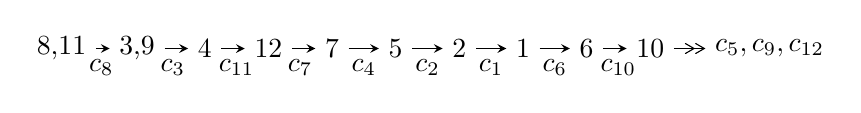
\begin{tikzpicture}[x=23pt, y=7pt]
	% node
	\node (A0) at (-1/8, 0) {8,11};
	\node (A1) at (17/16, 0) {3,9};
	\node (A2) at (17/8, 0) {4};
	\node (A3) at (25/8, 0) {12};
	\node (A4) at (33/8, 0) {7};
	\node (A5) at (41/8, 0) {5};
	\node (A6) at (49/8, 0) {2};
	\node (A7) at (57/8, 0) {1};
	\node (A8) at (65/8, 0) {6};
	\node (A9) at (73/8, 0) {10};
	\node (C1) at (1/2, -1) {$c_{8}$};
	\node (C2) at (13/8, -1) {$c_{3}$};
	\node (C3) at (21/8, -1) {$c_{11}$};
	\node (C4) at (29/8, -1) {$c_{7}$};
	\node (C5) at (37/8, -1) {$c_{4}$};
	\node (C6) at (45/8, -1) {$c_{2}$};
	\node (C7) at (53/8, -1) {$c_{1}$};
	\node (C8) at (61/8, -1) {$c_{6}$};
	\node (C9) at (69/8, -1) {$c_{10}$};
	\node (A10) at (11, 0) {$c_{5},c_{9},c_{12}$};

	% edge
	\draw[->,>=stealth]	
	(A0) edge (A1) (A1) edge (A2) (A2) edge (A3) (A3) edge (A4) (A4) edge (A5) (A5) edge (A6) (A6) edge (A7) (A7) edge (A8) (A8) edge (A9) ;
	\draw[->>,>={angle 60}]	
	(A9) edge (A10);
\end{tikzpicture} \\ 

\end{tabular} \\

\footnotetext{
The image of knot diagram is generated by the software ``\textbf{Draw programme}" developed by Andrew Bartholomew(\url{http://www.layer8.co.uk/maths/draw/index.htm\#Running-draw}), where we modified some parts for our purpose(\url{https://github.com/CATsTAILs/LinksPainter}).
}\phantom \\ \newline 
\centering \textbf{Ideals for irreducible components\footnotemark of $X_{\text{par}}$} 
 
\begin{align*}
I^u_{1}&=\langle 
- u^{21}+2 u^{20}+\cdots+2 b+2,\;3 u^{21}-14 u^{20}+\cdots+4 a-36,\;u^{22}-4 u^{21}+\cdots-22 u+4\rangle \\
I^u_{2}&=\langle 
2 u^{12}+u^{11}+10 u^{10}+3 u^9+15 u^8+u^7+3 u^6-4 u^5-3 u^4-4 u^3+5 u^2+b-2 u,\\
\phantom{I^u_{2}}&\phantom{= \langle  }-2 u^{10}-2 u^9-11 u^8-9 u^7-20 u^6-13 u^5-11 u^4-4 u^3+a+3 u-3,\\
\phantom{I^u_{2}}&\phantom{= \langle  }u^{13}+u^{12}+7 u^{11}+6 u^{10}+18 u^9+13 u^8+19 u^7+10 u^6+5 u^5-2 u^4- u^3-4 u^2+2 u+1\rangle \\
I^u_{3}&=\langle 
-4 a^3 u^2-19 a^3 u+8 a^2 u^2+9 a^3-17 a^2 u-8 u^2 a+4 a^2+28 a u-17 u^2+22 b-15 a- u-25,\\
\phantom{I^u_{3}}&\phantom{= \langle  }a^3 u^2+a^4+2 a^2 u^2+3 a^3+2 a^2 u+25 u^2 a+5 a^2+12 a u+15 u^2+55 a+7 u+33,\;u^3+2 u-1\rangle \\
I^u_{4}&=\langle 
-6 a^3 u^3-8 u^3 a^2+\cdots-27 a+12,\\
\phantom{I^u_{4}}&\phantom{= \langle  }2 a^3 u^3+a^3 u^2+u^3 a^2+a^4+4 a^3 u+a^2 u^2-4 u^3 a+a^3+a^2 u-5 u^2 a+2 u^3+2 a^2-4 a u+2 u^2-6 a+2 u,\\
\phantom{I^u_{4}}&\phantom{= \langle  }u^4+u^3+2 u^2+2 u+1\rangle \\
\\
\end{align*}
\raggedright * 4 irreducible components of $\dim_{\mathbb{C}}=0$, with total 63 representations.\\
\footnotetext{All coefficients of polynomials are rational numbers. But the coefficients are sometimes approximated in decimal forms when there is not enough margin.}
\newpage
\renewcommand{\arraystretch}{1}
\centering \section*{I. $I^u_{1}= \langle - u^{21}+2 u^{20}+\cdots+2 b+2,\;3 u^{21}-14 u^{20}+\cdots+4 a-36,\;u^{22}-4 u^{21}+\cdots-22 u+4 \rangle$}
\flushleft \textbf{(i) Arc colorings}\\
\begin{tabular}{m{7pt} m{180pt} m{7pt} m{180pt} }
\flushright $a_{8}=$&$\begin{pmatrix}1\\0\end{pmatrix}$ \\
\flushright $a_{11}=$&$\begin{pmatrix}0\\u\end{pmatrix}$ \\
\flushright $a_{3}=$&$\begin{pmatrix}-\frac{3}{4} u^{21}+\frac{7}{2} u^{20}+\cdots-\frac{151}{4} u+9\\\frac{1}{2} u^{21}- u^{20}+\cdots+\frac{3}{2} u-1\end{pmatrix}$ \\
\flushright $a_{9}=$&$\begin{pmatrix}1\\- u^2\end{pmatrix}$ \\
\flushright $a_{4}=$&$\begin{pmatrix}-\frac{5}{4} u^{21}+\frac{11}{2} u^{20}+\cdots-\frac{213}{4} u+12\\\frac{1}{2} u^{21}+2 u^{19}+\cdots-\frac{1}{2} u-1\end{pmatrix}$ \\
\flushright $a_{12}=$&$\begin{pmatrix}u\\u\end{pmatrix}$ \\
\flushright $a_{7}=$&$\begin{pmatrix}u^2+1\\u^2\end{pmatrix}$ \\
\flushright $a_{5}=$&$\begin{pmatrix}-\frac{3}{4} u^{21}+\frac{5}{2} u^{20}+\cdots-\frac{47}{4} u+1\\-\frac{1}{2} u^{21}+2 u^{20}+\cdots+\frac{31}{2} u-5\end{pmatrix}$ \\
\flushright $a_{2}=$&$\begin{pmatrix}-\frac{17}{4} u^{21}+\frac{29}{2} u^{20}+\cdots-\frac{289}{4} u+14\\-\frac{5}{2} u^{21}+10 u^{20}+\cdots-\frac{81}{2} u+7\end{pmatrix}$ \\
\flushright $a_{1}=$&$\begin{pmatrix}\frac{3}{2} u^{21}-\frac{11}{2} u^{20}+\cdots+\frac{73}{2} u-\frac{15}{2}\\\frac{1}{2} u^{21}-3 u^{20}+\cdots+\frac{27}{2} u-2\end{pmatrix}$ \\
\flushright $a_{6}=$&$\begin{pmatrix}-\frac{5}{2} u^{21}+\frac{17}{2} u^{20}+\cdots-\frac{83}{2} u+\frac{19}{2}\\-\frac{3}{2} u^{21}+6 u^{20}+\cdots-\frac{91}{2} u+10\end{pmatrix}$ \\
\flushright $a_{10}=$&$\begin{pmatrix}-\frac{1}{2} u^{20}+u^{19}+\cdots+7 u-\frac{3}{2}\\\frac{1}{2} u^{21}-2 u^{20}+\cdots+\frac{19}{2} u-2\end{pmatrix}$\\&\end{tabular}
\flushleft \textbf{(ii) Obstruction class $= -1$}\\~\\
\flushleft \textbf{(iii) Cusp Shapes $= -3 u^{21}+6 u^{20}-38 u^{19}+66 u^{18}-203 u^{17}+302 u^{16}-585 u^{15}+720 u^{14}-948 u^{13}+889 u^{12}-769 u^{11}+404 u^{10}-114 u^9-165 u^8+169 u^7-85 u^6-97 u^5+171 u^4-190 u^3+104 u^2-36 u-2$}\\~\\
\newpage\renewcommand{\arraystretch}{1}
\flushleft \textbf{(iv) u-Polynomials at the component}\newline \\
\begin{tabular}{m{50pt}|m{274pt}}
Crossings & \hspace{64pt}u-Polynomials at each crossing \\
\hline $$\begin{aligned}c_{1}\end{aligned}$$&$\begin{aligned}
&u^{22}+18 u^{21}+\cdots-4096 u+16384
\end{aligned}$\\
\hline $$\begin{aligned}c_{2},c_{6}\end{aligned}$$&$\begin{aligned}
&u^{22}-12 u^{21}+\cdots-576 u+128
\end{aligned}$\\
\hline $$\begin{aligned}c_{3},c_{5},c_{9}\\c_{10}\end{aligned}$$&$\begin{aligned}
&u^{22}- u^{20}+\cdots+u+1
\end{aligned}$\\
\hline $$\begin{aligned}c_{4},c_{12}\end{aligned}$$&$\begin{aligned}
&u^{22}+4 u^{21}+\cdots+u+1
\end{aligned}$\\
\hline $$\begin{aligned}c_{7},c_{8},c_{11}\end{aligned}$$&$\begin{aligned}
&u^{22}+4 u^{21}+\cdots+22 u+4
\end{aligned}$\\
\hline
\end{tabular}\\~\\
\newpage\renewcommand{\arraystretch}{1}
\flushleft \textbf{(v) Riley Polynomials at the component}\newline \\
\begin{tabular}{m{50pt}|m{274pt}}
Crossings & \hspace{64pt}Riley Polynomials at each crossing \\
\hline $$\begin{aligned}c_{1}\end{aligned}$$&$\begin{aligned}
&y^{22}-34 y^{21}+\cdots+83886080 y+268435456
\end{aligned}$\\
\hline $$\begin{aligned}c_{2},c_{6}\end{aligned}$$&$\begin{aligned}
&y^{22}-18 y^{21}+\cdots+4096 y+16384
\end{aligned}$\\
\hline $$\begin{aligned}c_{3},c_{5},c_{9}\\c_{10}\end{aligned}$$&$\begin{aligned}
&y^{22}-2 y^{21}+\cdots+5 y+1
\end{aligned}$\\
\hline $$\begin{aligned}c_{4},c_{12}\end{aligned}$$&$\begin{aligned}
&y^{22}+26 y^{21}+\cdots+53 y+1
\end{aligned}$\\
\hline $$\begin{aligned}c_{7},c_{8},c_{11}\end{aligned}$$&$\begin{aligned}
&y^{22}+20 y^{21}+\cdots+36 y+16
\end{aligned}$\\
\hline
\end{tabular}\\~\\
\newpage\flushleft \textbf{(vi) Complex Volumes and Cusp Shapes}
$$\begin{array}{c|c|c}  
\text{Solutions to }I^u_{1}& \I (\text{vol} + \sqrt{-1}CS) & \text{Cusp shape}\\
 \hline 
\begin{aligned}
u &= -0.113355 + 1.047390 I \\
a &= -0.249378 + 0.867554 I \\
b &= -0.12451 + 1.46269 I\end{aligned}
 & -0.89584 - 1.46775 I & -2.56568 + 4.64859 I \\ \hline\begin{aligned}
u &= -0.113355 - 1.047390 I \\
a &= -0.249378 - 0.867554 I \\
b &= -0.12451 - 1.46269 I\end{aligned}
 & -0.89584 + 1.46775 I & -2.56568 - 4.64859 I \\ \hline\begin{aligned}
u &= \phantom{-}0.616202 + 0.646773 I \\
a &= -1.102880 - 0.376255 I \\
b &= -1.397390 - 0.117675 I\end{aligned}
 & -7.62299 - 5.54296 I & -4.40972 + 2.06977 I \\ \hline\begin{aligned}
u &= \phantom{-}0.616202 - 0.646773 I \\
a &= -1.102880 + 0.376255 I \\
b &= -1.397390 + 0.117675 I\end{aligned}
 & -7.62299 + 5.54296 I & -4.40972 - 2.06977 I \\ \hline\begin{aligned}
u &= \phantom{-}0.764482 + 0.400206 I \\
a &= \phantom{-}0.05821 - 2.20084 I \\
b &= -0.292901 - 0.229775 I\end{aligned}
 & -6.80118 + 10.22180 I & -2.84650 - 6.91774 I \\ \hline\begin{aligned}
u &= \phantom{-}0.764482 - 0.400206 I \\
a &= \phantom{-}0.05821 + 2.20084 I \\
b &= -0.292901 + 0.229775 I\end{aligned}
 & -6.80118 - 10.22180 I & -2.84650 + 6.91774 I \\ \hline\begin{aligned}
u &= -0.761299 + 0.247632 I \\
a &= -0.069067 + 1.023690 I \\
b &= -0.281528 + 0.013910 I\end{aligned}
 & \phantom{-}1.16275 - 1.85731 I & \phantom{-}3.99806 - 0.12476 I \\ \hline\begin{aligned}
u &= -0.761299 - 0.247632 I \\
a &= -0.069067 - 1.023690 I \\
b &= -0.281528 - 0.013910 I\end{aligned}
 & \phantom{-}1.16275 + 1.85731 I & \phantom{-}3.99806 + 0.12476 I \\ \hline\begin{aligned}
u &= \phantom{-}0.686555 + 0.284442 I \\
a &= \phantom{-}0.25180 + 1.77617 I \\
b &= -0.119863 - 0.209977 I\end{aligned}
 & \phantom{-}0.31091 + 4.61412 I & -2.14647 - 8.90403 I \\ \hline\begin{aligned}
u &= \phantom{-}0.686555 - 0.284442 I \\
a &= \phantom{-}0.25180 - 1.77617 I \\
b &= -0.119863 + 0.209977 I\end{aligned}
 & \phantom{-}0.31091 - 4.61412 I & -2.14647 + 8.90403 I\\
 \hline 
 \end{array}$$\newpage$$\begin{array}{c|c|c}  
\text{Solutions to }I^u_{1}& \I (\text{vol} + \sqrt{-1}CS) & \text{Cusp shape}\\
 \hline 
\begin{aligned}
u &= \phantom{-}0.311371 + 0.544088 I \\
a &= -0.100430 + 0.264067 I \\
b &= \phantom{-}0.670256 + 0.493905 I\end{aligned}
 & -0.97447 - 1.03210 I & -5.19046 + 2.87964 I \\ \hline\begin{aligned}
u &= \phantom{-}0.311371 - 0.544088 I \\
a &= -0.100430 - 0.264067 I \\
b &= \phantom{-}0.670256 - 0.493905 I\end{aligned}
 & -0.97447 + 1.03210 I & -5.19046 - 2.87964 I \\ \hline\begin{aligned}
u &= -0.358815 + 1.338970 I \\
a &= \phantom{-}0.157826 - 0.737154 I \\
b &= \phantom{-}0.60731 - 1.77839 I\end{aligned}
 & -3.79504 - 5.99391 I & -0.31044 + 7.14857 I \\ \hline\begin{aligned}
u &= -0.358815 - 1.338970 I \\
a &= \phantom{-}0.157826 + 0.737154 I \\
b &= \phantom{-}0.60731 + 1.77839 I\end{aligned}
 & -3.79504 + 5.99391 I & -0.31044 - 7.14857 I \\ \hline\begin{aligned}
u &= \phantom{-}0.13972 + 1.42206 I \\
a &= \phantom{-}0.802494 + 0.162707 I \\
b &= \phantom{-}0.846933 - 0.294845 I\end{aligned}
 & -6.97755 + 0.69684 I & -7.99990 + 2.38959 I \\ \hline\begin{aligned}
u &= \phantom{-}0.13972 - 1.42206 I \\
a &= \phantom{-}0.802494 - 0.162707 I \\
b &= \phantom{-}0.846933 + 0.294845 I\end{aligned}
 & -6.97755 - 0.69684 I & -7.99990 - 2.38959 I \\ \hline\begin{aligned}
u &= \phantom{-}0.26914 + 1.41520 I \\
a &= -1.10275 - 1.22518 I \\
b &= -2.25955 - 2.13113 I\end{aligned}
 & -5.12121 + 8.09916 I & -6.73561 - 9.40400 I \\ \hline\begin{aligned}
u &= \phantom{-}0.26914 - 1.41520 I \\
a &= -1.10275 + 1.22518 I \\
b &= -2.25955 + 2.13113 I\end{aligned}
 & -5.12121 - 8.09916 I & -6.73561 + 9.40400 I \\ \hline\begin{aligned}
u &= \phantom{-}0.28842 + 1.47378 I \\
a &= \phantom{-}1.05609 + 1.33953 I \\
b &= \phantom{-}2.19735 + 3.10840 I\end{aligned}
 & -12.8364 + 14.0560 I & -6.34753 - 6.94319 I \\ \hline\begin{aligned}
u &= \phantom{-}0.28842 - 1.47378 I \\
a &= \phantom{-}1.05609 - 1.33953 I \\
b &= \phantom{-}2.19735 - 3.10840 I\end{aligned}
 & -12.8364 - 14.0560 I & -6.34753 + 6.94319 I\\
 \hline 
 \end{array}$$\newpage$$\begin{array}{c|c|c}  
\text{Solutions to }I^u_{1}& \I (\text{vol} + \sqrt{-1}CS) & \text{Cusp shape}\\
 \hline 
\begin{aligned}
u &= \phantom{-}0.15759 + 1.53295 I \\
a &= \phantom{-}0.048081 - 0.334870 I \\
b &= \phantom{-}1.153890 + 0.023955 I\end{aligned}
 & -14.8442 - 2.8448 I & -8.44574 + 2.22597 I \\ \hline\begin{aligned}
u &= \phantom{-}0.15759 - 1.53295 I \\
a &= \phantom{-}0.048081 + 0.334870 I \\
b &= \phantom{-}1.153890 - 0.023955 I\end{aligned}
 & -14.8442 + 2.8448 I & -8.44574 - 2.22597 I\\
 \hline 
 \end{array}$$\newpage\newpage\renewcommand{\arraystretch}{1}
\centering \section*{II. $I^u_{2}= \langle 2 u^{12}+u^{11}+\cdots+b-2 u,\;-2 u^{10}-2 u^9+\cdots+a-3,\;u^{13}+u^{12}+\cdots+2 u+1 \rangle$}
\flushleft \textbf{(i) Arc colorings}\\
\begin{tabular}{m{7pt} m{180pt} m{7pt} m{180pt} }
\flushright $a_{8}=$&$\begin{pmatrix}1\\0\end{pmatrix}$ \\
\flushright $a_{11}=$&$\begin{pmatrix}0\\u\end{pmatrix}$ \\
\flushright $a_{3}=$&$\begin{pmatrix}2 u^{10}+2 u^9+11 u^8+9 u^7+20 u^6+13 u^5+11 u^4+4 u^3-3 u+3\\-2 u^{12}- u^{11}+\cdots-5 u^2+2 u\end{pmatrix}$ \\
\flushright $a_{9}=$&$\begin{pmatrix}1\\- u^2\end{pmatrix}$ \\
\flushright $a_{4}=$&$\begin{pmatrix}- u^{11}+u^{10}+\cdots-5 u+3\\-2 u^{12}-2 u^{11}+\cdots- u^2-1\end{pmatrix}$ \\
\flushright $a_{12}=$&$\begin{pmatrix}u\\u\end{pmatrix}$ \\
\flushright $a_{7}=$&$\begin{pmatrix}u^2+1\\u^2\end{pmatrix}$ \\
\flushright $a_{5}=$&$\begin{pmatrix}u^{10}+u^9+6 u^8+5 u^7+12 u^6+8 u^5+8 u^4+3 u^3+u^2-2 u+2\\- u^{12}+u^{11}+\cdots-5 u^2+3 u\end{pmatrix}$ \\
\flushright $a_{2}=$&$\begin{pmatrix}u^{10}+u^9+6 u^8+5 u^7+12 u^6+8 u^5+8 u^4+4 u^3+u^2+2\\- u^{12}-5 u^{10}+u^9-7 u^8+4 u^7+4 u^5+2 u^4+2 u^3-4 u^2+3 u\end{pmatrix}$ \\
\flushright $a_{1}=$&$\begin{pmatrix}- u^{12}-8 u^{10}+\cdots+9 u-6\\2 u^{12}+2 u^{11}+\cdots- u^2+2\end{pmatrix}$ \\
\flushright $a_{6}=$&$\begin{pmatrix}u^{12}+u^{11}+7 u^{10}+5 u^9+17 u^8+8 u^7+15 u^6+2 u^5-6 u^3-2 u^2-5 u+3\\2 u^{11}+u^{10}+9 u^9+3 u^8+12 u^7+2 u^6+2 u^5-2 u^4- u^3-3 u^2+3 u-1\end{pmatrix}$ \\
\flushright $a_{10}=$&$\begin{pmatrix}u^{11}+u^{10}+6 u^9+5 u^8+13 u^7+9 u^6+11 u^5+5 u^4+2 u^3-2 u^2-2\\u^{12}+2 u^{11}+\cdots-2 u^2+1\end{pmatrix}$\\&\end{tabular}
\flushleft \textbf{(ii) Obstruction class $= 1$}\\~\\
\flushleft \textbf{(iii) Cusp Shapes $= -8 u^{12}-9 u^{11}-49 u^{10}-45 u^9-108 u^8-76 u^7-97 u^6-34 u^5-29 u^4+19 u^3-7 u^2+8 u-9$}\\~\\
\newpage\renewcommand{\arraystretch}{1}
\flushleft \textbf{(iv) u-Polynomials at the component}\newline \\
\begin{tabular}{m{50pt}|m{274pt}}
Crossings & \hspace{64pt}u-Polynomials at each crossing \\
\hline $$\begin{aligned}c_{1}\end{aligned}$$&$\begin{aligned}
&u^{13}-15 u^{12}+\cdots+33 u-4
\end{aligned}$\\
\hline $$\begin{aligned}c_{2}\end{aligned}$$&$\begin{aligned}
&u^{13}-3 u^{12}+\cdots+u-2
\end{aligned}$\\
\hline $$\begin{aligned}c_{3},c_{10}\end{aligned}$$&$\begin{aligned}
&u^{13}+5 u^{11}+u^{10}+7 u^9+4 u^8+4 u^6-4 u^5- u^4-2 u^2-1
\end{aligned}$\\
\hline $$\begin{aligned}c_{4},c_{12}\end{aligned}$$&$\begin{aligned}
&u^{13}-2 u^{12}+\cdots-4 u-1
\end{aligned}$\\
\hline $$\begin{aligned}c_{5},c_{9}\end{aligned}$$&$\begin{aligned}
&u^{13}+5 u^{11}- u^{10}+7 u^9-4 u^8-4 u^6-4 u^5+u^4+2 u^2+1
\end{aligned}$\\
\hline $$\begin{aligned}c_{6}\end{aligned}$$&$\begin{aligned}
&u^{13}+3 u^{12}+\cdots+u+2
\end{aligned}$\\
\hline $$\begin{aligned}c_{7},c_{8}\end{aligned}$$&$\begin{aligned}
&u^{13}+u^{12}+\cdots+2 u+1
\end{aligned}$\\
\hline $$\begin{aligned}c_{11}\end{aligned}$$&$\begin{aligned}
&u^{13}- u^{12}+\cdots+2 u-1
\end{aligned}$\\
\hline
\end{tabular}\\~\\
\newpage\renewcommand{\arraystretch}{1}
\flushleft \textbf{(v) Riley Polynomials at the component}\newline \\
\begin{tabular}{m{50pt}|m{274pt}}
Crossings & \hspace{64pt}Riley Polynomials at each crossing \\
\hline $$\begin{aligned}c_{1}\end{aligned}$$&$\begin{aligned}
&y^{13}-27 y^{12}+\cdots-79 y-16
\end{aligned}$\\
\hline $$\begin{aligned}c_{2},c_{6}\end{aligned}$$&$\begin{aligned}
&y^{13}-15 y^{12}+\cdots+33 y-4
\end{aligned}$\\
\hline $$\begin{aligned}c_{3},c_{5},c_{9}\\c_{10}\end{aligned}$$&$\begin{aligned}
&y^{13}+10 y^{12}+\cdots-4 y-1
\end{aligned}$\\
\hline $$\begin{aligned}c_{4},c_{12}\end{aligned}$$&$\begin{aligned}
&y^{13}-10 y^{12}+\cdots-4 y-1
\end{aligned}$\\
\hline $$\begin{aligned}c_{7},c_{8},c_{11}\end{aligned}$$&$\begin{aligned}
&y^{13}+13 y^{12}+\cdots+12 y-1
\end{aligned}$\\
\hline
\end{tabular}\\~\\
\newpage\flushleft \textbf{(vi) Complex Volumes and Cusp Shapes}
$$\begin{array}{c|c|c}  
\text{Solutions to }I^u_{2}& \I (\text{vol} + \sqrt{-1}CS) & \text{Cusp shape}\\
 \hline 
\begin{aligned}
u &= -0.773550 + 0.446076 I \\
a &= -0.305684 + 0.776454 I \\
b &= -0.221370 + 0.094049 I\end{aligned}
 & \phantom{-}1.27688 - 2.47819 I & \phantom{-}8.06933 + 11.56907 I \\ \hline\begin{aligned}
u &= -0.773550 - 0.446076 I \\
a &= -0.305684 - 0.776454 I \\
b &= -0.221370 - 0.094049 I\end{aligned}
 & \phantom{-}1.27688 + 2.47819 I & \phantom{-}8.06933 - 11.56907 I \\ \hline\begin{aligned}
u &= \phantom{-}0.098733 + 1.212320 I \\
a &= \phantom{-}1.13507 + 1.02542 I \\
b &= \phantom{-}1.70497 + 2.47623 I\end{aligned}
 & \phantom{-}1.58553 + 1.07079 I & \phantom{-}1.79491 + 0.89145 I \\ \hline\begin{aligned}
u &= \phantom{-}0.098733 - 1.212320 I \\
a &= \phantom{-}1.13507 - 1.02542 I \\
b &= \phantom{-}1.70497 - 2.47623 I\end{aligned}
 & \phantom{-}1.58553 - 1.07079 I & \phantom{-}1.79491 - 0.89145 I \\ \hline\begin{aligned}
u &= -0.125906 + 1.364640 I \\
a &= -1.26556 - 0.79157 I \\
b &= -1.18557 - 2.02372 I\end{aligned}
 & -8.30588 - 1.59896 I & -12.80035 + 0.14504 I \\ \hline\begin{aligned}
u &= -0.125906 - 1.364640 I \\
a &= -1.26556 + 0.79157 I \\
b &= -1.18557 + 2.02372 I\end{aligned}
 & -8.30588 + 1.59896 I & -12.80035 - 0.14504 I \\ \hline\begin{aligned}
u &= \phantom{-}0.218616 + 1.386220 I \\
a &= -1.009230 - 0.765658 I \\
b &= -2.45521 - 2.30542 I\end{aligned}
 & -0.64678 + 3.91620 I & -4.73840 - 4.05034 I \\ \hline\begin{aligned}
u &= \phantom{-}0.218616 - 1.386220 I \\
a &= -1.009230 + 0.765658 I \\
b &= -2.45521 + 2.30542 I\end{aligned}
 & -0.64678 - 3.91620 I & -4.73840 + 4.05034 I \\ \hline\begin{aligned}
u &= \phantom{-}0.542233 + 0.204630 I \\
a &= \phantom{-}0.95589 + 2.90373 I \\
b &= \phantom{-}0.500761 + 0.448666 I\end{aligned}
 & \phantom{-}4.46035 + 1.08841 I & \phantom{-}0.69467 - 6.25717 I \\ \hline\begin{aligned}
u &= \phantom{-}0.542233 - 0.204630 I \\
a &= \phantom{-}0.95589 - 2.90373 I \\
b &= \phantom{-}0.500761 - 0.448666 I\end{aligned}
 & \phantom{-}4.46035 - 1.08841 I & \phantom{-}0.69467 + 6.25717 I\\
 \hline 
 \end{array}$$\newpage$$\begin{array}{c|c|c}  
\text{Solutions to }I^u_{2}& \I (\text{vol} + \sqrt{-1}CS) & \text{Cusp shape}\\
 \hline 
\begin{aligned}
u &= -0.30546 + 1.45345 I \\
a &= \phantom{-}0.544780 - 0.691123 I \\
b &= \phantom{-}1.25789 - 1.48118 I\end{aligned}
 & -4.73020 - 6.43920 I & -5.54584 + 8.97180 I \\ \hline\begin{aligned}
u &= -0.30546 - 1.45345 I \\
a &= \phantom{-}0.544780 + 0.691123 I \\
b &= \phantom{-}1.25789 + 1.48118 I\end{aligned}
 & -4.73020 + 6.43920 I & -5.54584 - 8.97180 I \\ \hline\begin{aligned}
u &= -0.309328\phantom{ +0.000000I} \\
a &= \phantom{-}3.88946\phantom{ +0.000000I} \\
b &= -1.20295\phantom{ +0.000000I}\end{aligned}
 & -3.72913\phantom{ +0.000000I} & -12.9490\phantom{ +0.000000I}\\
 \hline 
 \end{array}$$\newpage\newpage\renewcommand{\arraystretch}{1}
\centering \section*{III. $I^u_{3}= \langle -4 a^3 u^2+8 a^2 u^2+\cdots-15 a-25,\;a^3 u^2+2 a^2 u^2+\cdots+55 a+33,\;u^3+2 u-1 \rangle$}
\flushleft \textbf{(i) Arc colorings}\\
\begin{tabular}{m{7pt} m{180pt} m{7pt} m{180pt} }
\flushright $a_{8}=$&$\begin{pmatrix}1\\0\end{pmatrix}$ \\
\flushright $a_{11}=$&$\begin{pmatrix}0\\u\end{pmatrix}$ \\
\flushright $a_{3}=$&$\begin{pmatrix}a\\0.181818 a^{3} u^{2}-0.363636 a^{2} u^{2}+\cdots+0.681818 a+1.13636\end{pmatrix}$ \\
\flushright $a_{9}=$&$\begin{pmatrix}1\\- u^2\end{pmatrix}$ \\
\flushright $a_{4}=$&$\begin{pmatrix}-0.181818 a^{3} u^{2}+0.363636 a^{2} u^{2}+\cdots+0.318182 a-1.13636\\-0.590909 a^{3} u^{2}+0.181818 a^{2} u^{2}+\cdots-0.590909 a+1.18182\end{pmatrix}$ \\
\flushright $a_{12}=$&$\begin{pmatrix}u\\u\end{pmatrix}$ \\
\flushright $a_{7}=$&$\begin{pmatrix}u^2+1\\u^2\end{pmatrix}$ \\
\flushright $a_{5}=$&$\begin{pmatrix}0.181818 a^{3} u^{2}-0.363636 a^{2} u^{2}+\cdots+0.681818 a+1.13636\\-\frac{1}{2} a^3 u^2-\frac{3}{2} a^2 u^2+\cdots- a+\frac{3}{2}\end{pmatrix}$ \\
\flushright $a_{2}=$&$\begin{pmatrix}1.04545 a^{3} u^{2}+0.409091 a^{2} u^{2}+\cdots+2.04545 a+1.90909\\1.81818 a^{3} u^{2}-0.136364 a^{2} u^{2}+\cdots+2.31818 a+1.86364\end{pmatrix}$ \\
\flushright $a_{1}=$&$\begin{pmatrix}0.727273 a^{3} u^{2}+0.0454545 a^{2} u^{2}+\cdots+0.727273 a+2.54545\\a^3 u^2-\frac{1}{2} u^2 a+\cdots+a-1\end{pmatrix}$ \\
\flushright $a_{6}=$&$\begin{pmatrix}-1.36364 a^{3} u^{2}-0.772727 a^{2} u^{2}+\cdots-1.36364 a-1.27273\\-2.27273 a^{3} u^{2}-0.454545 a^{2} u^{2}+\cdots-2.27273 a-2.45455\end{pmatrix}$ \\
\flushright $a_{10}=$&$\begin{pmatrix}-0.136364 a^{3} u^{2}+0.272727 a^{2} u^{2}+\cdots-0.136364 a+0.272727\\0.272727 a^{3} u^{2}+1.45455 a^{2} u^{2}+\cdots+0.272727 a+1.45455\end{pmatrix}$\\&\end{tabular}
\flushleft \textbf{(ii) Obstruction class $= -1$}\\~\\
\flushleft \textbf{(iii) Cusp Shapes $= 4 u^2+4 u+2$}\\~\\
\newpage\renewcommand{\arraystretch}{1}
\flushleft \textbf{(iv) u-Polynomials at the component}\newline \\
\begin{tabular}{m{50pt}|m{274pt}}
Crossings & \hspace{64pt}u-Polynomials at each crossing \\
\hline $$\begin{aligned}c_{1}\end{aligned}$$&$\begin{aligned}
&(u^2+3 u+1)^6
\end{aligned}$\\
\hline $$\begin{aligned}c_{2},c_{6}\end{aligned}$$&$\begin{aligned}
&(u^2+u-1)^6
\end{aligned}$\\
\hline $$\begin{aligned}c_{3},c_{5},c_{9}\\c_{10}\end{aligned}$$&$\begin{aligned}
&u^{12}+u^{10}+u^9+6 u^8+6 u^7+8 u^6+20 u^5+4 u^4+7 u^3+19 u^2+2 u-4
\end{aligned}$\\
\hline $$\begin{aligned}c_{4},c_{12}\end{aligned}$$&$\begin{aligned}
&u^{12}+2 u^{11}+\cdots-18 u+44
\end{aligned}$\\
\hline $$\begin{aligned}c_{7},c_{8},c_{11}\end{aligned}$$&$\begin{aligned}
&(u^3+2 u+1)^4
\end{aligned}$\\
\hline
\end{tabular}\\~\\
\newpage\renewcommand{\arraystretch}{1}
\flushleft \textbf{(v) Riley Polynomials at the component}\newline \\
\begin{tabular}{m{50pt}|m{274pt}}
Crossings & \hspace{64pt}Riley Polynomials at each crossing \\
\hline $$\begin{aligned}c_{1}\end{aligned}$$&$\begin{aligned}
&(y^2-7 y+1)^6
\end{aligned}$\\
\hline $$\begin{aligned}c_{2},c_{6}\end{aligned}$$&$\begin{aligned}
&(y^2-3 y+1)^6
\end{aligned}$\\
\hline $$\begin{aligned}c_{3},c_{5},c_{9}\\c_{10}\end{aligned}$$&$\begin{aligned}
&y^{12}+2 y^{11}+\cdots-156 y+16
\end{aligned}$\\
\hline $$\begin{aligned}c_{4},c_{12}\end{aligned}$$&$\begin{aligned}
&y^{12}+6 y^{11}+\cdots+820 y+1936
\end{aligned}$\\
\hline $$\begin{aligned}c_{7},c_{8},c_{11}\end{aligned}$$&$\begin{aligned}
&(y^3+4 y^2+4 y-1)^4
\end{aligned}$\\
\hline
\end{tabular}\\~\\
\newpage\flushleft \textbf{(vi) Complex Volumes and Cusp Shapes}
$$\begin{array}{c|c|c}  
\text{Solutions to }I^u_{3}& \I (\text{vol} + \sqrt{-1}CS) & \text{Cusp shape}\\
 \hline 
\begin{aligned}
u &= -0.22670 + 1.46771 I \\
a &= \phantom{-}0.854692 - 0.614486 I \\
b &= \phantom{-}1.58719 - 1.61371 I\end{aligned}
 & -5.49289 - 5.13794 I & -7.31793 + 3.20902 I \\ \hline\begin{aligned}
u &= -0.22670 + 1.46771 I \\
a &= -0.263183 - 0.362701 I \\
b &= -1.65920 + 0.15080 I\end{aligned}
 & -13.3886 - 5.1379 I & -7.31793 + 3.20902 I \\ \hline\begin{aligned}
u &= -0.22670 + 1.46771 I \\
a &= -0.300182 + 0.203211 I \\
b &= -0.007380 + 0.210795 I\end{aligned}
 & -5.49289 - 5.13794 I & -7.31793 + 3.20902 I \\ \hline\begin{aligned}
u &= -0.22670 + 1.46771 I \\
a &= -1.18854 + 1.43943 I \\
b &= -2.47679 + 3.52208 I\end{aligned}
 & -13.3886 - 5.1379 I & -7.31793 + 3.20902 I \\ \hline\begin{aligned}
u &= -0.22670 - 1.46771 I \\
a &= \phantom{-}0.854692 + 0.614486 I \\
b &= \phantom{-}1.58719 + 1.61371 I\end{aligned}
 & -5.49289 + 5.13794 I & -7.31793 - 3.20902 I \\ \hline\begin{aligned}
u &= -0.22670 - 1.46771 I \\
a &= -0.263183 + 0.362701 I \\
b &= -1.65920 - 0.15080 I\end{aligned}
 & -13.3886 + 5.1379 I & -7.31793 - 3.20902 I \\ \hline\begin{aligned}
u &= -0.22670 - 1.46771 I \\
a &= -0.300182 - 0.203211 I \\
b &= -0.007380 - 0.210795 I\end{aligned}
 & -5.49289 + 5.13794 I & -7.31793 - 3.20902 I \\ \hline\begin{aligned}
u &= -0.22670 - 1.46771 I \\
a &= -1.18854 - 1.43943 I \\
b &= -2.47679 - 3.52208 I\end{aligned}
 & -13.3886 + 5.1379 I & -7.31793 - 3.20902 I \\ \hline\begin{aligned}
u &= \phantom{-}0.453398\phantom{ +0.000000I} \\
a &= -0.626782\phantom{ +0.000000I} \\
b &= \phantom{-}1.23526\phantom{ +0.000000I}\end{aligned}
 & -3.16064\phantom{ +0.000000I} & \phantom{-}4.63590\phantom{ +0.000000I} \\ \hline\begin{aligned}
u &= \phantom{-}0.453398\phantom{ +0.000000I} \\
a &= \phantom{-}0.99058 + 3.57131 I \\
b &= -0.343740 + 0.608968 I\end{aligned}
 & \phantom{-}4.73504\phantom{ +0.000000I} & \phantom{-}4.63590\phantom{ +0.000000I}\\
 \hline 
 \end{array}$$\newpage$$\begin{array}{c|c|c}  
\text{Solutions to }I^u_{3}& \I (\text{vol} + \sqrt{-1}CS) & \text{Cusp shape}\\
 \hline 
\begin{aligned}
u &= \phantom{-}0.453398\phantom{ +0.000000I} \\
a &= \phantom{-}0.99058 - 3.57131 I \\
b &= -0.343740 - 0.608968 I\end{aligned}
 & \phantom{-}4.73504\phantom{ +0.000000I} & \phantom{-}4.63590\phantom{ +0.000000I} \\ \hline\begin{aligned}
u &= \phantom{-}0.453398\phantom{ +0.000000I} \\
a &= -4.55994\phantom{ +0.000000I} \\
b &= \phantom{-}0.564588\phantom{ +0.000000I}\end{aligned}
 & -3.16064\phantom{ +0.000000I} & \phantom{-}4.63590\phantom{ +0.000000I}\\
 \hline 
 \end{array}$$\newpage\newpage\renewcommand{\arraystretch}{1}
\centering \section*{IV. $I^u_{4}= \langle -6 a^3 u^3-8 u^3 a^2+\cdots-27 a+12,\;2 a^3 u^3+u^3 a^2+\cdots+2 a^2-6 a,\;u^4+u^3+2 u^2+2 u+1 \rangle$}
\flushleft \textbf{(i) Arc colorings}\\
\begin{tabular}{m{7pt} m{180pt} m{7pt} m{180pt} }
\flushright $a_{8}=$&$\begin{pmatrix}1\\0\end{pmatrix}$ \\
\flushright $a_{11}=$&$\begin{pmatrix}0\\u\end{pmatrix}$ \\
\flushright $a_{3}=$&$\begin{pmatrix}a\\0.176471 a^{3} u^{3}+0.235294 a^{2} u^{3}+\cdots+0.794118 a-0.352941\end{pmatrix}$ \\
\flushright $a_{9}=$&$\begin{pmatrix}1\\- u^2\end{pmatrix}$ \\
\flushright $a_{4}=$&$\begin{pmatrix}-0.176471 a^{3} u^{3}-0.235294 a^{2} u^{3}+\cdots+0.205882 a+0.352941\\0.264706 a^{2} u^{3}-0.264706 a u^{3}+\cdots+0.441176 a-0.764706\end{pmatrix}$ \\
\flushright $a_{12}=$&$\begin{pmatrix}u\\u\end{pmatrix}$ \\
\flushright $a_{7}=$&$\begin{pmatrix}u^2+1\\u^2\end{pmatrix}$ \\
\flushright $a_{5}=$&$\begin{pmatrix}-0.558824 a^{3} u^{3}+0.676471 a^{2} u^{3}+\cdots-0.117647 a+0.529412\\-0.0882353 a^{3} u^{3}+0.500000 a^{2} u^{3}+\cdots-0.117647 a+0.0588235\end{pmatrix}$ \\
\flushright $a_{2}=$&$\begin{pmatrix}-0.117647 a^{3} u^{3}+0.647059 a^{2} u^{3}+\cdots+2.58824 a-0.235294\\0.0588235 a^{3} u^{3}+0.617647 a^{2} u^{3}+\cdots+0.941176 a+0.176471\end{pmatrix}$ \\
\flushright $a_{1}=$&$\begin{pmatrix}0.0294118 a^{3} u^{3}+0.0882353 a^{2} u^{3}+\cdots+0.852941 a+0.0588235\\-0.147059 a^{3} u^{3}+0.294118 a^{2} u^{3}+\cdots-0.705882 a+0.470588\end{pmatrix}$ \\
\flushright $a_{6}=$&$\begin{pmatrix}0.264706 a^{3} u^{3}-1.20588 a^{2} u^{3}+\cdots-2.32353 a+0.529412\\\frac{3}{34} a^3 u^3-\frac{8}{17} u^3 a^2+\cdots- a-\frac{10}{17}\end{pmatrix}$ \\
\flushright $a_{10}=$&$\begin{pmatrix}-0.294118 a^{2} u^{3}+0.294118 a u^{3}+\cdots+0.676471 a+1.29412\\-0.117647 a^{3} u^{3}-0.176471 a^{2} u^{3}+\cdots+0.882353 a+0.588235\end{pmatrix}$\\&\end{tabular}
\flushleft \textbf{(ii) Obstruction class $= -1$}\\~\\
\flushleft \textbf{(iii) Cusp Shapes $= 4 u^3+4 u-2$}\\~\\
\newpage\renewcommand{\arraystretch}{1}
\flushleft \textbf{(iv) u-Polynomials at the component}\newline \\
\begin{tabular}{m{50pt}|m{274pt}}
Crossings & \hspace{64pt}u-Polynomials at each crossing \\
\hline $$\begin{aligned}c_{1}\end{aligned}$$&$\begin{aligned}
&(u^2+3 u+1)^8
\end{aligned}$\\
\hline $$\begin{aligned}c_{2},c_{6}\end{aligned}$$&$\begin{aligned}
&(u^2+u-1)^8
\end{aligned}$\\
\hline $$\begin{aligned}c_{3},c_{5},c_{9}\\c_{10}\end{aligned}$$&$\begin{aligned}
&u^{16}- u^{15}+\cdots-4 u+1
\end{aligned}$\\
\hline $$\begin{aligned}c_{4},c_{12}\end{aligned}$$&$\begin{aligned}
&u^{16}+5 u^{15}+\cdots+50 u+19
\end{aligned}$\\
\hline $$\begin{aligned}c_{7},c_{8},c_{11}\end{aligned}$$&$\begin{aligned}
&(u^4- u^3+2 u^2-2 u+1)^4
\end{aligned}$\\
\hline
\end{tabular}\\~\\
\newpage\renewcommand{\arraystretch}{1}
\flushleft \textbf{(v) Riley Polynomials at the component}\newline \\
\begin{tabular}{m{50pt}|m{274pt}}
Crossings & \hspace{64pt}Riley Polynomials at each crossing \\
\hline $$\begin{aligned}c_{1}\end{aligned}$$&$\begin{aligned}
&(y^2-7 y+1)^8
\end{aligned}$\\
\hline $$\begin{aligned}c_{2},c_{6}\end{aligned}$$&$\begin{aligned}
&(y^2-3 y+1)^8
\end{aligned}$\\
\hline $$\begin{aligned}c_{3},c_{5},c_{9}\\c_{10}\end{aligned}$$&$\begin{aligned}
&y^{16}+5 y^{15}+\cdots-8 y+1
\end{aligned}$\\
\hline $$\begin{aligned}c_{4},c_{12}\end{aligned}$$&$\begin{aligned}
&y^{16}-7 y^{15}+\cdots-752 y+361
\end{aligned}$\\
\hline $$\begin{aligned}c_{7},c_{8},c_{11}\end{aligned}$$&$\begin{aligned}
&(y^4+3 y^3+2 y^2+1)^4
\end{aligned}$\\
\hline
\end{tabular}\\~\\
\newpage\flushleft \textbf{(vi) Complex Volumes and Cusp Shapes}
$$\begin{array}{c|c|c}  
\text{Solutions to }I^u_{4}& \I (\text{vol} + \sqrt{-1}CS) & \text{Cusp shape}\\
 \hline 
\begin{aligned}
u &= -0.621744 + 0.440597 I \\
a &= -0.542830 + 1.141380 I \\
b &= -0.231778 + 0.327115 I\end{aligned}
 & \phantom{-}0.65797 - 2.02988 I & -4.00000 + 3.46410 I \\ \hline\begin{aligned}
u &= -0.621744 + 0.440597 I \\
a &= \phantom{-}1.35588 - 0.69513 I \\
b &= \phantom{-}1.316260 - 0.130390 I\end{aligned}
 & -7.23771 - 2.02988 I & -4.00000 + 3.46410 I \\ \hline\begin{aligned}
u &= -0.621744 + 0.440597 I \\
a &= -0.106754 + 0.135093 I \\
b &= -0.417805 - 0.121114 I\end{aligned}
 & \phantom{-}0.65797 - 2.02988 I & -4.00000 + 3.46410 I \\ \hline\begin{aligned}
u &= -0.621744 + 0.440597 I \\
a &= \phantom{-}0.34475 - 2.64671 I \\
b &= \phantom{-}0.384377 - 0.408927 I\end{aligned}
 & -7.23771 - 2.02988 I & -4.00000 + 3.46410 I \\ \hline\begin{aligned}
u &= -0.621744 - 0.440597 I \\
a &= -0.542830 - 1.141380 I \\
b &= -0.231778 - 0.327115 I\end{aligned}
 & \phantom{-}0.65797 + 2.02988 I & -4.00000 - 3.46410 I \\ \hline\begin{aligned}
u &= -0.621744 - 0.440597 I \\
a &= \phantom{-}1.35588 + 0.69513 I \\
b &= \phantom{-}1.316260 + 0.130390 I\end{aligned}
 & -7.23771 + 2.02988 I & -4.00000 - 3.46410 I \\ \hline\begin{aligned}
u &= -0.621744 - 0.440597 I \\
a &= -0.106754 - 0.135093 I \\
b &= -0.417805 + 0.121114 I\end{aligned}
 & \phantom{-}0.65797 + 2.02988 I & -4.00000 - 3.46410 I \\ \hline\begin{aligned}
u &= -0.621744 - 0.440597 I \\
a &= \phantom{-}0.34475 + 2.64671 I \\
b &= \phantom{-}0.384377 + 0.408927 I\end{aligned}
 & -7.23771 + 2.02988 I & -4.00000 - 3.46410 I \\ \hline\begin{aligned}
u &= \phantom{-}0.121744 + 1.306620 I \\
a &= \phantom{-}0.904436 - 0.255157 I \\
b &= \phantom{-}0.193308 - 0.950380 I\end{aligned}
 & -7.23771 + 2.02988 I & -4.00000 - 3.46410 I \\ \hline\begin{aligned}
u &= \phantom{-}0.121744 + 1.306620 I \\
a &= \phantom{-}0.630729 + 1.205030 I \\
b &= \phantom{-}1.45960 + 3.32611 I\end{aligned}
 & \phantom{-}0.65797 + 2.02988 I & -4.00000 - 3.46410 I\\
 \hline 
 \end{array}$$\newpage$$\begin{array}{c|c|c}  
\text{Solutions to }I^u_{4}& \I (\text{vol} + \sqrt{-1}CS) & \text{Cusp shape}\\
 \hline 
\begin{aligned}
u &= \phantom{-}0.121744 + 1.306620 I \\
a &= -1.52623 - 0.46379 I \\
b &= -2.35510 - 1.51441 I\end{aligned}
 & \phantom{-}0.65797 + 2.02988 I & -4.00000 - 3.46410 I \\ \hline\begin{aligned}
u &= \phantom{-}0.121744 + 1.306620 I \\
a &= \phantom{-}1.44002 - 1.68542 I \\
b &= \phantom{-}2.15115 - 3.79271 I\end{aligned}
 & -7.23771 + 2.02988 I & -4.00000 - 3.46410 I \\ \hline\begin{aligned}
u &= \phantom{-}0.121744 - 1.306620 I \\
a &= \phantom{-}0.904436 + 0.255157 I \\
b &= \phantom{-}0.193308 + 0.950380 I\end{aligned}
 & -7.23771 - 2.02988 I & -4.00000 + 3.46410 I \\ \hline\begin{aligned}
u &= \phantom{-}0.121744 - 1.306620 I \\
a &= \phantom{-}0.630729 - 1.205030 I \\
b &= \phantom{-}1.45960 - 3.32611 I\end{aligned}
 & \phantom{-}0.65797 - 2.02988 I & -4.00000 + 3.46410 I \\ \hline\begin{aligned}
u &= \phantom{-}0.121744 - 1.306620 I \\
a &= -1.52623 + 0.46379 I \\
b &= -2.35510 + 1.51441 I\end{aligned}
 & \phantom{-}0.65797 - 2.02988 I & -4.00000 + 3.46410 I \\ \hline\begin{aligned}
u &= \phantom{-}0.121744 - 1.306620 I \\
a &= \phantom{-}1.44002 + 1.68542 I \\
b &= \phantom{-}2.15115 + 3.79271 I\end{aligned}
 & -7.23771 - 2.02988 I & -4.00000 + 3.46410 I\\
 \hline 
 \end{array}$$\newpage
\newpage\renewcommand{\arraystretch}{1}
\centering \section*{ V. u-Polynomials}
\begin{tabular}{m{50pt}|m{274pt}}
Crossings & \hspace{64pt}u-Polynomials at each crossing \\
\hline $$\begin{aligned}c_{1}\end{aligned}$$&$\begin{aligned}
&((u^2+3 u+1)^{14})(u^{13}-15 u^{12}+\cdots+33 u-4)\\
&\cdot(u^{22}+18 u^{21}+\cdots-4096 u+16384)
\end{aligned}$\\
\hline $$\begin{aligned}c_{2}\end{aligned}$$&$\begin{aligned}
&((u^2+u-1)^{14})(u^{13}-3 u^{12}+\cdots+u-2)\\
&\cdot(u^{22}-12 u^{21}+\cdots-576 u+128)
\end{aligned}$\\
\hline $$\begin{aligned}c_{3},c_{10}\end{aligned}$$&$\begin{aligned}
&(u^{12}+u^{10}+u^9+6 u^8+6 u^7+8 u^6+20 u^5+4 u^4+7 u^3+19 u^2+2 u-4)\\
&\cdot(u^{13}+5 u^{11}+u^{10}+7 u^9+4 u^8+4 u^6-4 u^5- u^4-2 u^2-1)\\
&\cdot(u^{16}- u^{15}+\cdots-4 u+1)(u^{22}- u^{20}+\cdots+u+1)
\end{aligned}$\\
\hline $$\begin{aligned}c_{4},c_{12}\end{aligned}$$&$\begin{aligned}
&(u^{12}+2 u^{11}+\cdots-18 u+44)(u^{13}-2 u^{12}+\cdots-4 u-1)\\
&\cdot(u^{16}+5 u^{15}+\cdots+50 u+19)(u^{22}+4 u^{21}+\cdots+u+1)
\end{aligned}$\\
\hline $$\begin{aligned}c_{5},c_{9}\end{aligned}$$&$\begin{aligned}
&(u^{12}+u^{10}+u^9+6 u^8+6 u^7+8 u^6+20 u^5+4 u^4+7 u^3+19 u^2+2 u-4)\\
&\cdot(u^{13}+5 u^{11}- u^{10}+7 u^9-4 u^8-4 u^6-4 u^5+u^4+2 u^2+1)\\
&\cdot(u^{16}- u^{15}+\cdots-4 u+1)(u^{22}- u^{20}+\cdots+u+1)
\end{aligned}$\\
\hline $$\begin{aligned}c_{6}\end{aligned}$$&$\begin{aligned}
&((u^2+u-1)^{14})(u^{13}+3 u^{12}+\cdots+u+2)\\
&\cdot(u^{22}-12 u^{21}+\cdots-576 u+128)
\end{aligned}$\\
\hline $$\begin{aligned}c_{7},c_{8}\end{aligned}$$&$\begin{aligned}
&((u^3+2 u+1)^4)(u^4- u^3+2 u^2-2 u+1)^{4}(u^{13}+u^{12}+\cdots+2 u+1)\\
&\cdot(u^{22}+4 u^{21}+\cdots+22 u+4)
\end{aligned}$\\
\hline $$\begin{aligned}c_{11}\end{aligned}$$&$\begin{aligned}
&((u^3+2 u+1)^4)(u^4- u^3+2 u^2-2 u+1)^{4}(u^{13}- u^{12}+\cdots+2 u-1)\\
&\cdot(u^{22}+4 u^{21}+\cdots+22 u+4)
\end{aligned}$\\
\hline
\end{tabular}\newpage\renewcommand{\arraystretch}{1}
\centering \section*{ VI. Riley Polynomials}
\begin{tabular}{m{50pt}|m{274pt}}
Crossings & \hspace{64pt}Riley Polynomials at each crossing \\
\hline $$\begin{aligned}c_{1}\end{aligned}$$&$\begin{aligned}
&((y^2-7 y+1)^{14})(y^{13}-27 y^{12}+\cdots-79 y-16)\\
&\cdot(y^{22}-34 y^{21}+\cdots+83886080 y+268435456)
\end{aligned}$\\
\hline $$\begin{aligned}c_{2},c_{6}\end{aligned}$$&$\begin{aligned}
&((y^2-3 y+1)^{14})(y^{13}-15 y^{12}+\cdots+33 y-4)\\
&\cdot(y^{22}-18 y^{21}+\cdots+4096 y+16384)
\end{aligned}$\\
\hline $$\begin{aligned}c_{3},c_{5},c_{9}\\c_{10}\end{aligned}$$&$\begin{aligned}
&(y^{12}+2 y^{11}+\cdots-156 y+16)(y^{13}+10 y^{12}+\cdots-4 y-1)\\
&\cdot(y^{16}+5 y^{15}+\cdots-8 y+1)(y^{22}-2 y^{21}+\cdots+5 y+1)
\end{aligned}$\\
\hline $$\begin{aligned}c_{4},c_{12}\end{aligned}$$&$\begin{aligned}
&(y^{12}+6 y^{11}+\cdots+820 y+1936)(y^{13}-10 y^{12}+\cdots-4 y-1)\\
&\cdot(y^{16}-7 y^{15}+\cdots-752 y+361)(y^{22}+26 y^{21}+\cdots+53 y+1)
\end{aligned}$\\
\hline $$\begin{aligned}c_{7},c_{8},c_{11}\end{aligned}$$&$\begin{aligned}
&(y^3+4 y^2+4 y-1)^4(y^4+3 y^3+2 y^2+1)^4\\
&\cdot(y^{13}+13 y^{12}+\cdots+12 y-1)(y^{22}+20 y^{21}+\cdots+36 y+16)
\end{aligned}$\\
\hline
\end{tabular}
\vskip 2pc
\end{document}